\section{Qualitative assessment: interpretability}
\label{sec:opint:qualitative}
This section presents a qualitative assessment of the clustering performances based on the interpretability of the discovered groups of messages.
In particular, the discussion is articulated by simulating the shifter's perspective when reading the pipeline outputs.
In the following, we report five cherry-picked examples to showcase our approach's major successes and failures.
Specifically, we first illustrate a thorough examination of the biggest cluster discovered (see \cref{fig:cluster_summary:successes}, cluster with $\text{id}=0$).
Then we highlight some strengths and limitations of our approach, bringing other exemplary cases as evidence.
The same procedure and similar conclusions apply likewise to most groups. Thus, a complete dissertation is omitted here for conciseness\footnote{full results \opintresults}.

% The individual outputs of our pipeline constitutes two alternative starting points for the investigation.
% Although the summary table would be an equally valid option, the suggested strategy is to prefer the time evolution charts instead.
% In fact, the former output may be more demanding and challenging. On the contrary, time plots clearly illustrate the magnitude of the problem and its trend.


The main output of our pipeline is the summary table illustrated in \cref{fig:cluster_summary:successes,fig:cluster_summary:failures}, which reports a succinct highlight of the cluster contents and represents the most substantial source of information.
A reasonable reading approach is to start with the groups including more errors and gradually proceed with the smaller ones.
In this case, the biggest cluster is shown in \cref{fig:cluster_summary:successes} in the first row with $\text{id}=0$.
Despite including almost 820k error strings (\textbox{\# cluster size}), the actual number of different messages is only 117%
%, as testified by the \textbox{\# strings} statistics.
 (\textbox{\# strings}).
This number further reduces to simply 14 unique patterns (\textbox{\# patterns}) after the abstraction mechanism described in \cref{sec:viz} is applied, which is way more manageable for manual inspection than the initial cluster size.
% This observation suggests that the pipeline has learned something similar to the abstraction mechanism.
% % The previous hypothesis is also confirmed by the \textbox{message} column, where the raw strings differ only by the \textbox{\$URL} and \textbox{\$ADDRESS} parameters.
% Indeed, the raw error strings differ only by the \textbox{\$URL} and \textbox{\$ADDRESS} parameters (see \textbox{message} column).
% The same
% This property is highly desirable in practice, as it testifies that the approach produces a good embedded representation and recognizes the similarity of messages sharing the same raw strings up to some parametric parts. 
% This result, in turn, corroborates the initial design choice of applying minimal pre-processing and letting the model learn by itself.
A second insight is then provided by the \textit{Top-3} section. 
Including the auxiliary information about the source and destination sites involved makes it evident as the failures are united by the same error template and destination site.
This suggests that \texttt{Site-4} may have a problem and that its root cause is linked to the error pattern reported in the \textbox{message} column. 
Finally, the last piece of information to consider is the time evolution plot (see \cref{fig:timeplots:growing}). 
In this case, the cluster shows an increasing trend throughout the whole day of analysis. Specifically, the number of generated failures grows from less than 2000 errors at the beginning of the day to a value around five times higher, with an incremented boost from 9 a.m. onwards.
By and large, all these factors clearly advise that a potential issue is happening at \texttt{Site-4} as it always appears as a destination. 
Also, the message information further suggests that the failure is linked to a \textit{revoked certificate} that cannot be verified.
Finally, the time chart shows that the problem is escalating and need prompt intervention.

Despite providing only good proxies of the actual end goals -- i.e. \textit{root causes} and \textit{solving actions} --, this rapid analysis already points to actionable insights regarding \textit{where} and \textit{what} faults occur and whether they represent a real concern.
Notice that one can draw similar conclusions by looking separately at the site transfer efficiency and the most frequent unique strings or patterns. 
However, observing high failure rates for \texttt{Site-4} only answers to \textit{where} the faults occur. 
Likewise, the information contained in the errors only relates to the \textit{what} part of the question.
Thus, both approaches would lead to partial conclusions and require additional investigations to reach the same result.
Conversely, our approach addresses the two tasks together, thus letting the conclusion emerge rapidly and naturally. 
Remarkably, a further advantage is that one can leverage both site and pattern information for more precise indications.
For instance, one could hypothesize that not only the \texttt{Site-4} is experiencing a problem, but the issue is limited to incoming connections. Indeed, \texttt{Site-4} is involved only as a destination, and the error patterns point to something related to \textbox{destination overwrite}.
Therefore, the previous advantages show how shifting from the current site-centric focus to a hybrid strategy based on error messages and auxiliary information is beneficial.
\begin{landscape}
\begin{figure}
    \centering
    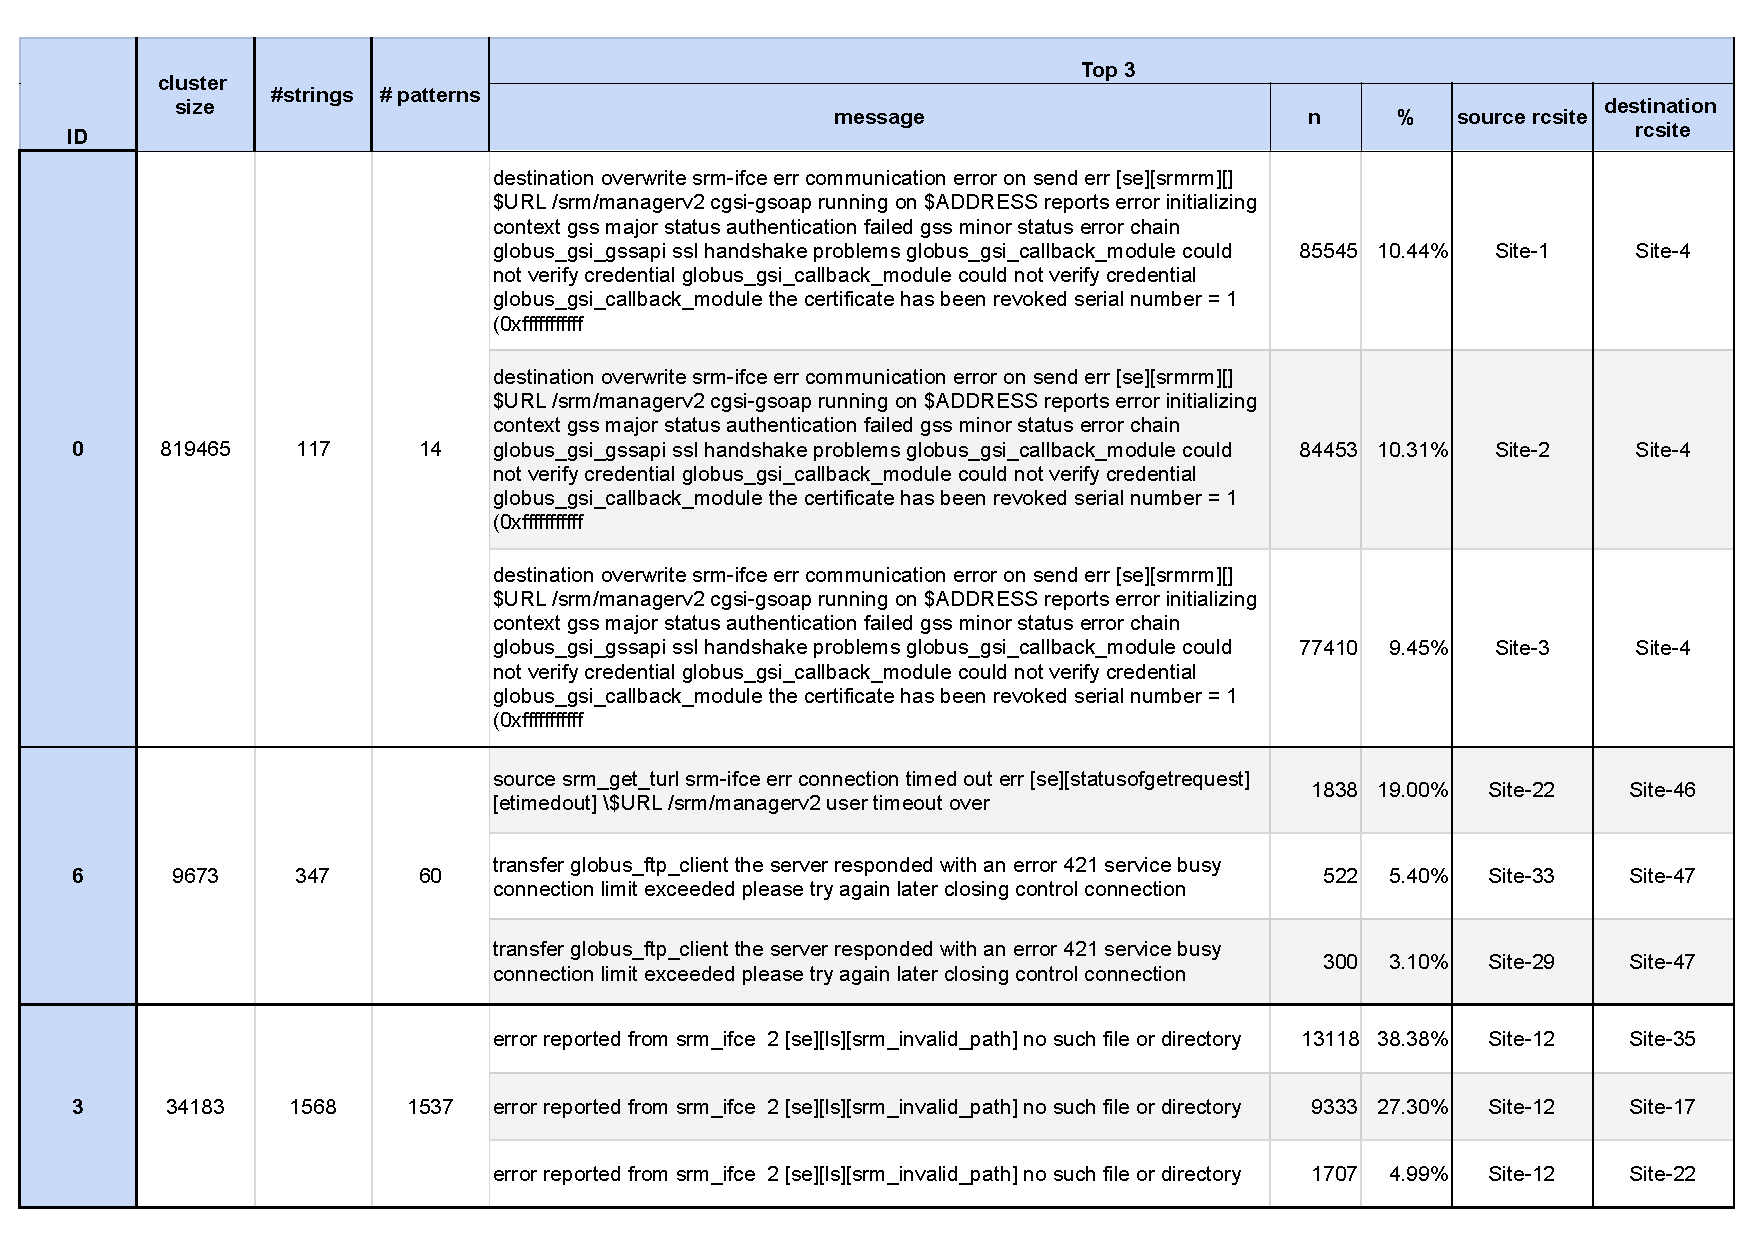
\includegraphics[width=\linewidth]{figures/510_results/cluster-summary-successes.pdf}
    \caption{\textbf{Summary table: successes.}
    The figure illustrates the main achievements of the pipeline. 
    Cluster 3 provides immediate indication of the error type (pattern) and where it occurs.
    The others also suggest the approach is actually learning to understand message parameters (cluster 0) and message semantic (cluster 6)
    % , at least to some extent.
    % The first 3 columns contain numeric summaries of the cluster composition. The \textit{Top-3} section draw a high-level overview of the cluster content summed up by the most frequently observed error triplets of error pattern, source and destination.
    }
    \label{fig:cluster_summary:successes}
\end{figure}
\end{landscape}

In addition to the practical usage of our pipeline, the results illustrated in \cref{fig:cluster_summary:successes,fig:cluster_summary:failures} expose interesting insights about what the models are actually learning.
For instance, the substantial reduction observed passing from errors to patterns suggests that the pipeline has learned something similar to an abstraction mechanism.
% The previous hypothesis is also confirmed by the \textbox{message} column, where the raw strings differ only by the \textbox{\$URL} and \textbox{\$ADDRESS} parameters.
Indeed, the raw error strings of \textbox{cluster 0} differ only by the \textbox{\$URL} and \textbox{\$ADDRESS} parameters (see \textbox{message} column).
Although one may argue that the same could be obtained using a flexible parsing strategy, the superiority of our approach is even more evident in \textbox{cluster 6} (\cref{fig:cluster_summary:successes}). 
In this case, the clustering joins two patterns with a far less straightforward linkage.
In fact, this result appears to resemble the human association that \textbox{connection timed out} (first pattern) may be linked to a \textbox{service busy connection limit exceeded} (second and third) problem.
Notably, this is a much higher level of abstraction with respect to a smart parsing approach, and it goes way beyond what one could achieve based on good abstraction heuristics.
Clearly, this property is remarkable and highly desirable in practice, as it testifies that the approach produces a good embedded representation and recognizes the similarity of messages sharing similar content.
In particular, this holds not only up to some parametric parts but also in terms of their actual meaning.
% the same raw strings up to some parametric parts. 
In turn, this observation corroborates the initial design choice of applying minimal pre-processing and letting the model learn by itself.

Another clear example of success is provided by the \textbox{cluster 3} (\cref{fig:cluster_summary:successes}), where the visualization makes it immediate for the shifter to understand that the issue is related to a missing file (\textbox{no such file or directory}) at \textbox{Site-12}.

However, our pipeline comes also with some limitations (\cref{fig:cluster_summary:failures}). 
For instance, the two patterns reported in \textbox{cluster 4} show a more vague connection that would require more in-depth investigation.
As a matter of fact, they seem to be linked due to a generic \textbox{server responded with an error} which is a very generic incipit to several error strings. Apart from that, the error codes are different (\textbox{[3021]} VS \textbox{[3010]}, which may imply the clustering is too coarse and a more refined distinction is needed.
Also, the messages point to seemingly extraneous issues (storage VS authentication).
Such observations expose two limitations. On the one hand, tuning the pipeline to meet the desired level of granularity when separating different groups is extremely complex. 
%In practice, just increasing the number of clusters may be insufficient as it does not allow to select where the split should happen.
On the other hand, this behavior may be due to the difficulty in comparing longer strings (first and second patterns) with short-text (third).

Another drawback is related to how outliers are handled. The k-means algorithm is bounded to the specified number of clusters, $k$, which sets the number of output groups irrespective of the underlying structure of the data.
As a result, the outliers are often incorporated into the closer cluster. When the latter is big enough, they probably pass undetected as they are dispersed into un heap of other messages. However, they may contaminate other clusters when the affected group has a comparable size, as in the case of second and third patterns in \textbox{cluster 2}.

\begin{landscape}
\begin{figure}
    \centering
    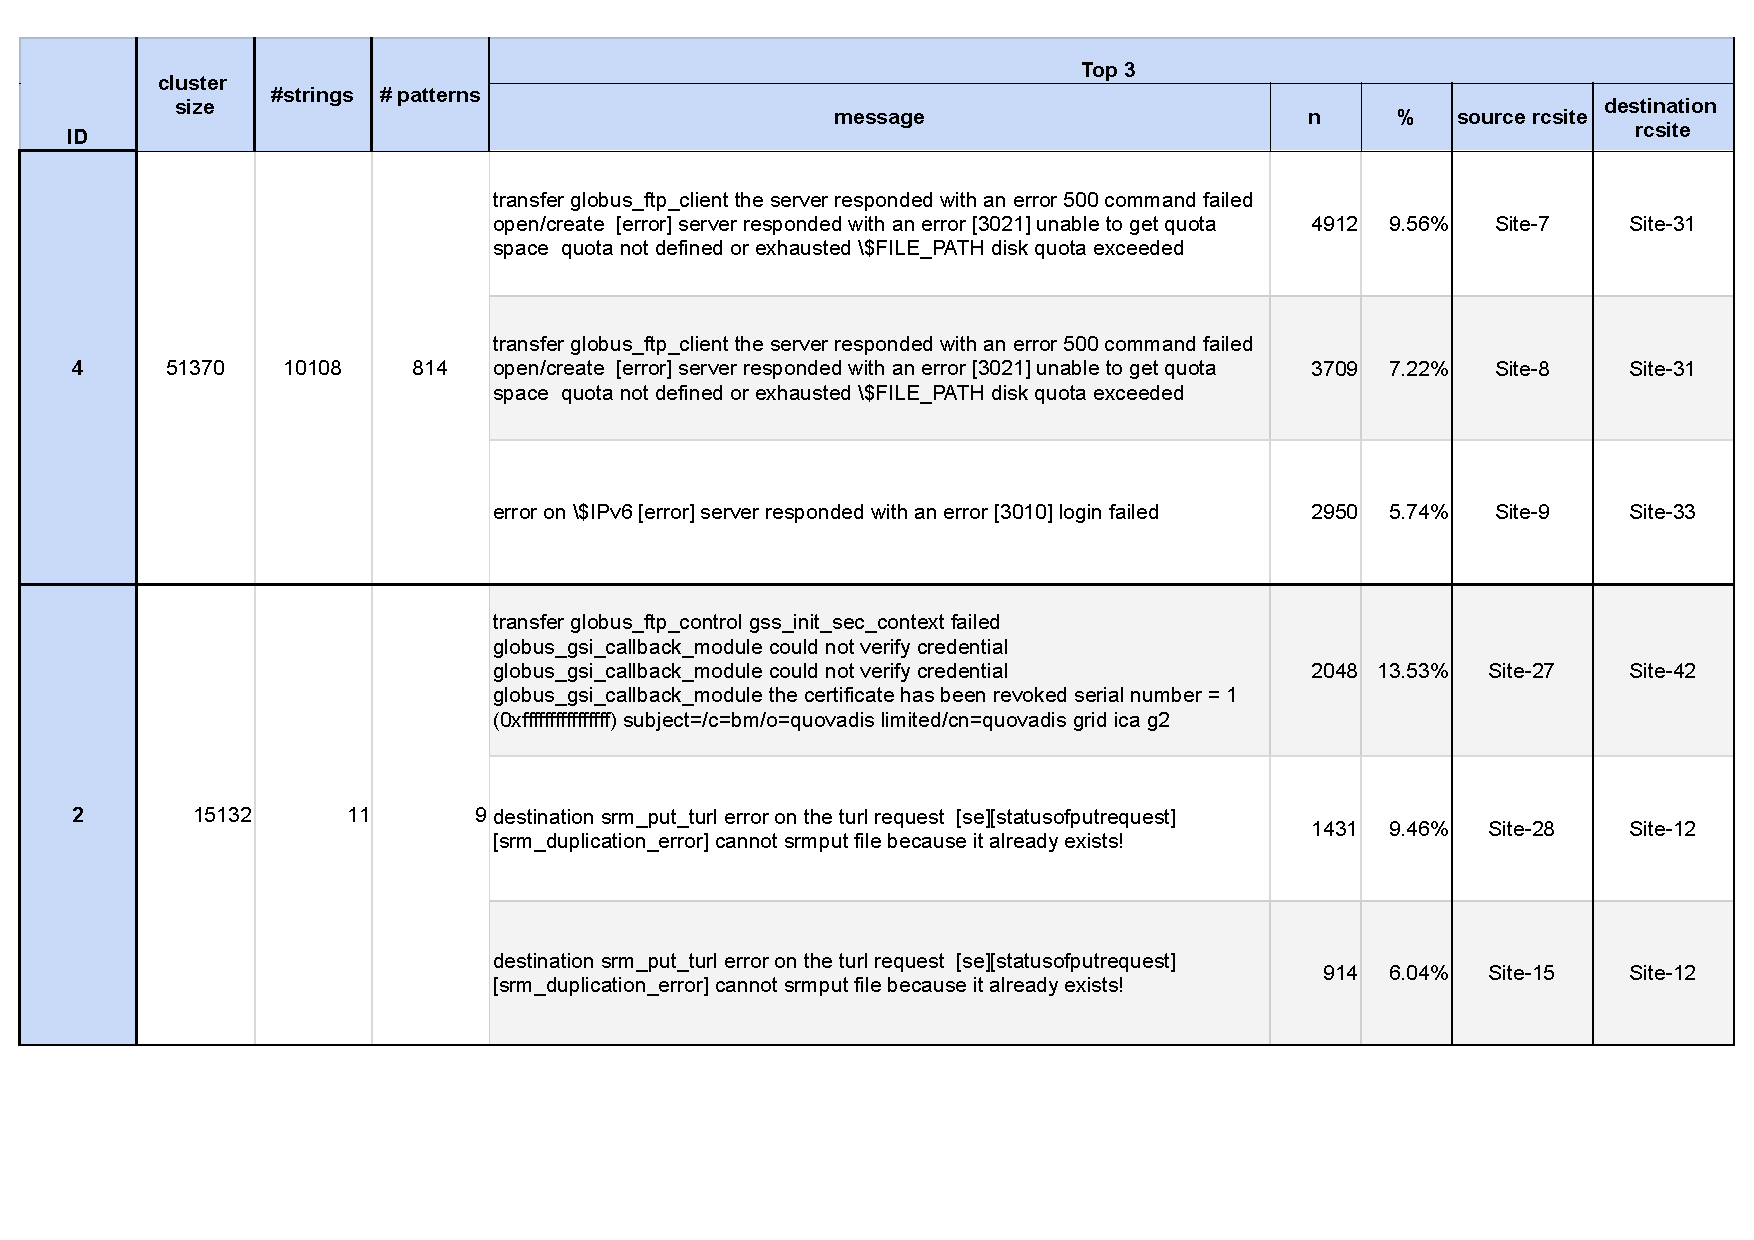
\includegraphics[width=\linewidth]{figures/510_results/cluster-summary-failures.pdf}
    \caption{\textbf{Summary table: limitations.}
    The two clusters show evidence of contaminated groups due to generic partial matching (cluster 4) or outliers aggregation (cluster 2)
    }
    \label{fig:cluster_summary:failures}
\end{figure}
\end{landscape}

% \begin{landscape}
%     \begin{figure}
%         \centering
%         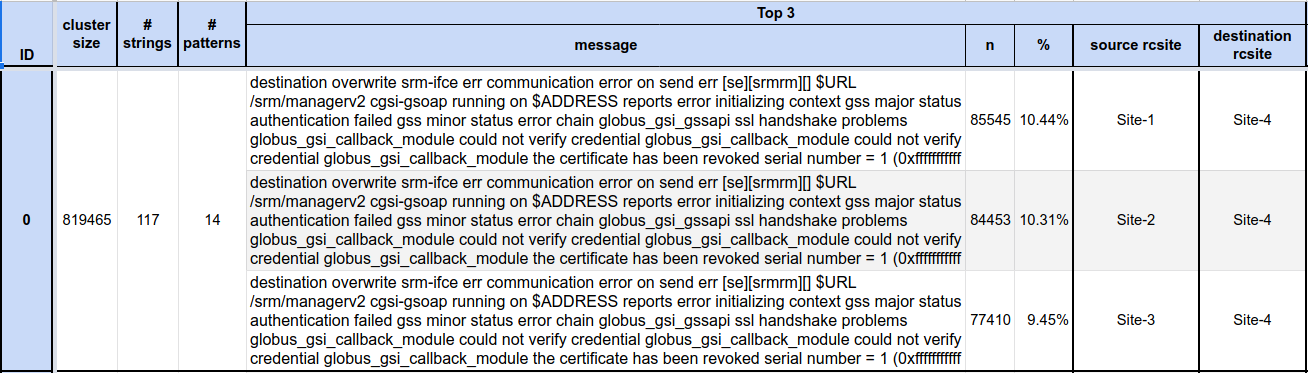
\includegraphics[width=\linewidth]{figures/510_results/cluster0_wide.png}
%         \caption{ \textbf{Example cluster summary.}
%         The first 3 columns contain numeric summaries of the cluster composition. The \textit{Top-3} section draw a high-level overview of the cluster content summed up by the most frequently observed error triplets of error pattern, source and destination.
%         }
%         \label{fig:cluster0}
%     \end{figure}
% \end{landscape}
% \begin{landscape}
%     \begin{figure}
%         \centering
%         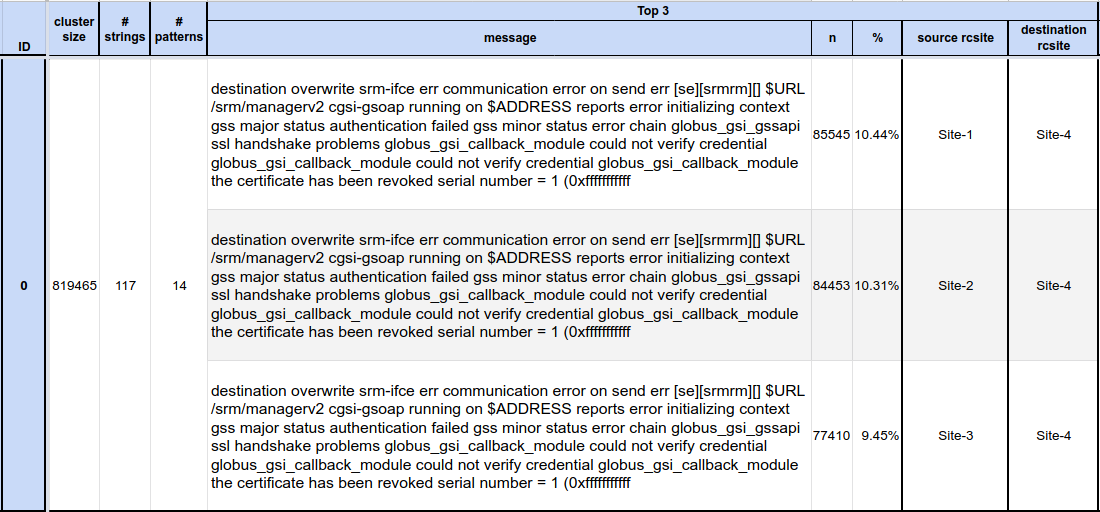
\includegraphics[width=\linewidth]{figures/510_results/cluster0_table.png}
%         \caption{ \textbf{Example cluster summary.}
%         The first 3 columns contain numeric summaries of the cluster composition. The \textit{Top-3} section draw a high-level overview of the cluster content summed up by the most frequently observed error triplets of error pattern, source and destination.
%         }
%         \label{fig:cluster0}
%     \end{figure}
% \end{landscape}

% \begin{landscape}
% \begin{figure}
%     \centering
%     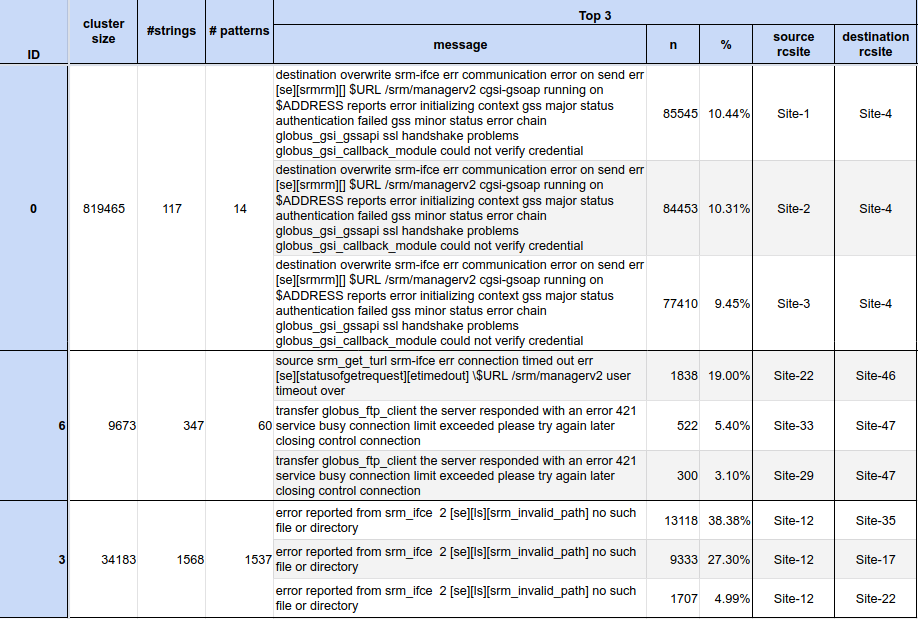
\includegraphics[width=\linewidth]{figures/510_results/timeplots/table-successes.png}
%     \caption{Caption}
%     \label{fig:cluster_summary:successes}
% \end{figure}
% \end{landscape}

% \begin{landscape}
% \begin{figure}
%     \centering
%     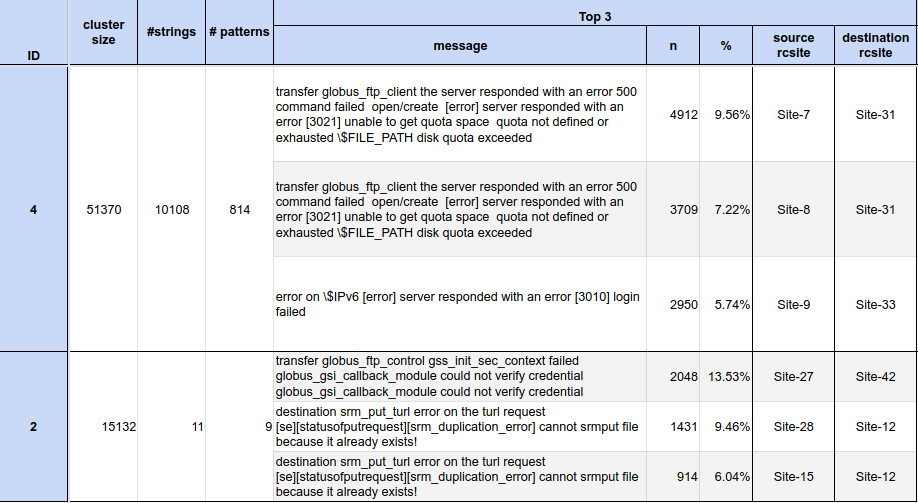
\includegraphics[width=\linewidth]{figures/510_results/timeplots/table-failures.png}
%     \caption{Caption}
%     \label{fig:cluster_summary:failures}
% \end{figure}
% \end{landscape}